\documentclass[a4paper,british,oneside,12pt]{scrartcl}
\usepackage[bshspec]{bshstyle2}

\usepackage{hyperref}
\usepackage{graphicx}
%\usepackage{lastpage}
\usepackage{longtable}
\usepackage{supertabular}
\usepackage{isodate}
%\usepackage{babel}
\usepackage{tabulary}
\usepackage{hyperref}
\usepackage{colortbl}
\usepackage[strings]{underscore}
\usepackage{pst-uml}
\usepackage{listings}
\usepackage{framed}
\usepackage{pdflscape}
%Use \us for '_' as original is so ugly
%\newcommand{\us}{\hspace{0.3em}\_\hspace{-0.8em}\_\hspace{0.2em}}
\def\us{\kern.08em\vbox{\hrule width.35em height.6pt}\kern.08em}

\definecolor{RuHo}{rgb}{0.5,0,1}
\definecolor{jele}{rgb}{.6,0.4,.75}

%\remark{JeLe}{my remark}
%\remark{RuHo}{Runes remark}


\newcolumntype{F}{>{\columncolor[gray]{.92}\centering\footnotesize}m{1.05cm}}
\newcolumntype{B}{>{\color{white}\columncolor[gray]{.38}\centering\footnotesize}m{1.05cm}}
\newcolumntype{L}{>{\centering}m{1pt}}
\newcolumntype{X}{>{\centering}m{4pt}}
\newcolumntype{D}{>{\centering\footnotesize $\cdots$} m{4mm}}
\newlength{\tabcolsepBak}
\newlength{\arrayrulewidthBak}
\setlength{\tabcolsepBak}{\tabcolsep}
\setlength{\arrayrulewidthBak}{\arrayrulewidth}


\newcommand{\mkMsgFrame}[4][]{
\setlength\tabcolsep{1pt}
\renewcommand\arraystretch{1.3}
\setlength\arrayrulewidth{1pt}
 \vspace{8pt}
 \noindent
 \begin{tabular}
   {X|#2|X}
  	\hline
  	& #3 &\tabularnewline
  	#4
  	#1
 \end{tabular}
 \vspace{8pt}
 \setlength\tabcolsep{\tabcolsepBak}
 \renewcommand\arraystretch{1.0}
 \setlength\arrayrulewidth{\arrayrulewidthBak}
}


\renewcommand\pdmTitle{          Boot Loader Specification}
\renewcommand\pdmDescr{          This document specifies the BSH~GED Boot Loader}
\renewcommand\pdmVersion{        1.9}
\renewcommand\pdmStatus{         Released}
\renewcommand\pdmIndex{          --}
\renewcommand\pdmEco{            --}
\renewcommand\pdmDocNo{          --}
\renewcommand\pdmAuthor{         Jens Lehmann}
\renewcommand\pdmEmail{          Jens.Lehmann@bshg.com}
\renewcommand\pdmCreationDate{   12.11.2009}
\renewcommand\pdmLastAmendment{  Jens Lehmann}
\renewcommand\pdmAmendmentDate{  \today}
\renewcommand\pdmDocType{        Specification}
\renewcommand\pdmDocAbstact{%
  This document specifies the rough design of boot loader application and the protocol.}


\newcommand{\bl}{\emph{BL}}
\newcommand{\fp}{\emph{FP}}
\newcommand{\dbus}{\emph{DBus2}}
\newcommand{\bra}{\emph{BRA}}
\newcommand{\bro}{\emph{BRO}}
\newcommand{\bp}{\emph{BP}} % Boot Programmer, discuss name (all in one loader)
\newcommand{\uc}{$\mu$C}


\begin{document}
\makePdmTitle

\tableofcontents
\newpage
\pagestyle{scrheadings}


\section*{Revision history}

\makeRevHistory{%
1.0 			& Setup new document based on ``Bootloader design and protocol'' (55600000003810).	& Jens Lehmann	& 24.11.2009\\
1.1       & Rework, all commands specified & Jens Lehmann & 14.12.2009\\
1.2       & Commands SET_BAUDRATE and BREAK adapted & Jens Lehmann & 09.03.2010\\
1.3       & Command SET_BAUDRATE adapted, ADL is used instead of ADH if just a single byte is required  & Jens Lehmann & 29.04.2010\\
1.4       & Chapter Overview added & Jens Lehmann & 28.09.2010\\
1.5       & Chapter Data Length added (Special meaning of data length zero defined)\\
          & New empty chapter 'Naming Convention' added & Jens Lehmann & 04.11.2010\\
1.6       & New chapter 'Communication settings' added\\
          & Buffered writing extended\\
          & Differences and new chapter reviewed (Holen/Lehmann)  & Jens Lehmann & 08.04.2011\\
          & Review and release & Jens Lehmann\\
					& 									 & Rune Holen & 25.05.2012\\
1.7       & Command for CRC calculation added & Jens Lehmann & 10.06.2014\\
1.8       & Firmware Update Chapter added & Alexander Kiefl & 25.06.2019\\
1.9       & Chapter 'Bootloader Transition State Chart' updated. Chapter 'Buffered Mode' removed & Jens Lehmann & 23.12.2020
}



\section{Introduction}
This document describes the rough Boot Loader (\bl{}) design and the interaction with the application in an embedded system and with the Flash Programmer (\fp{}).

\subsection{Aim}
Without defining implementation details this document specifies all required details to develop a \bl{}-App\-li\-ca\-tion for any embedded platform.

\subsection{Limitations}
This document does not define or discuss any implementation details. As it should enable a sub-contractor of BSH also to develop a \bl{} which works together with the GED Flash Programmer \fp{}. The \bl{} has been designed for wired firmware update, never the less the \bl{} may also be included in a system which provides remote firmware update (chapter \ref{sec:FirmwareUpdate}).

\newpage
\subsection{Coexisting Documents}
Please note, that some of the following documents are for internal use only, they are not valid for BSH sub-contractor.\\

\makeCoexistingDocs{%
1 & Software Naming Convention       & NamingConvention.doc & EDS:A915.AAAA-DOCU\\
2 & Software Coding Rules            & CodingRules.pdf      & EDS:A14.AAAA-GL\\
3 & Universal Flash Programmer       & ApplicationSpecifications.doc & \\
4 & BSH General Bus Specification D-Bus-2 & D-BusII.pdf & 5560 0000003459\\
}


\subsection{Terms and Abbreviations}

\makeTerms{%
BL          & Boot Loader\\
BRA         & RAM-Loader: This part of \bl{} will be uploaded into RAM of micro controller by the \fp{}.
              It is an application containing the routines for programming and erasing flash memory.\\
BRO         & ROM-Loader: The memory resistant part of \bl{}, responsible for handling startup sequence
              and receiving the RAM-Loader application.\\
LRO         & Loadable ROM-Loader. This application does the same as the ROM-Loader, but it is not the root application if the \uc{}, it will be started by a Boot Manager.\\
BP          & Boot-Programmer: This application is a ROM-Loader containing also the flash routines.
              This is required, if the \uc{}-Platform does not support execution of code inside RAM.\\
D-Bus-2       & Unified bus system used in BSH household appliances, one-wire and UART based\\
ECU         & Electronic Control Unit\\
FP          & Flash~Programmer: A tool communicating with the Boot Loader for programming the $\mu{}C$\\
ID-String   & String saved in the ROM-\bl{} holds information about the \uc{}-Platform, \bl{} and optional about the project.\\
CRC         & The Cyclic redundancy check is a mathematical method commonly used in digital networks and storage devices to detect accidental changes to raw data.
 
}

\newpage

\section{Overall View}
To programme the nonvolatile memory of an embedded system there are different applications required. In order to programme different devices in different systems the hardware of D-Bus-2 is used. This interface is unified and available in nearly every BSH household appliance with electronic controls\footnote{The older standard diagnostic can be used as well, but not for higher baud rates}.\\

\begin{figure}[ht]
	\centering
		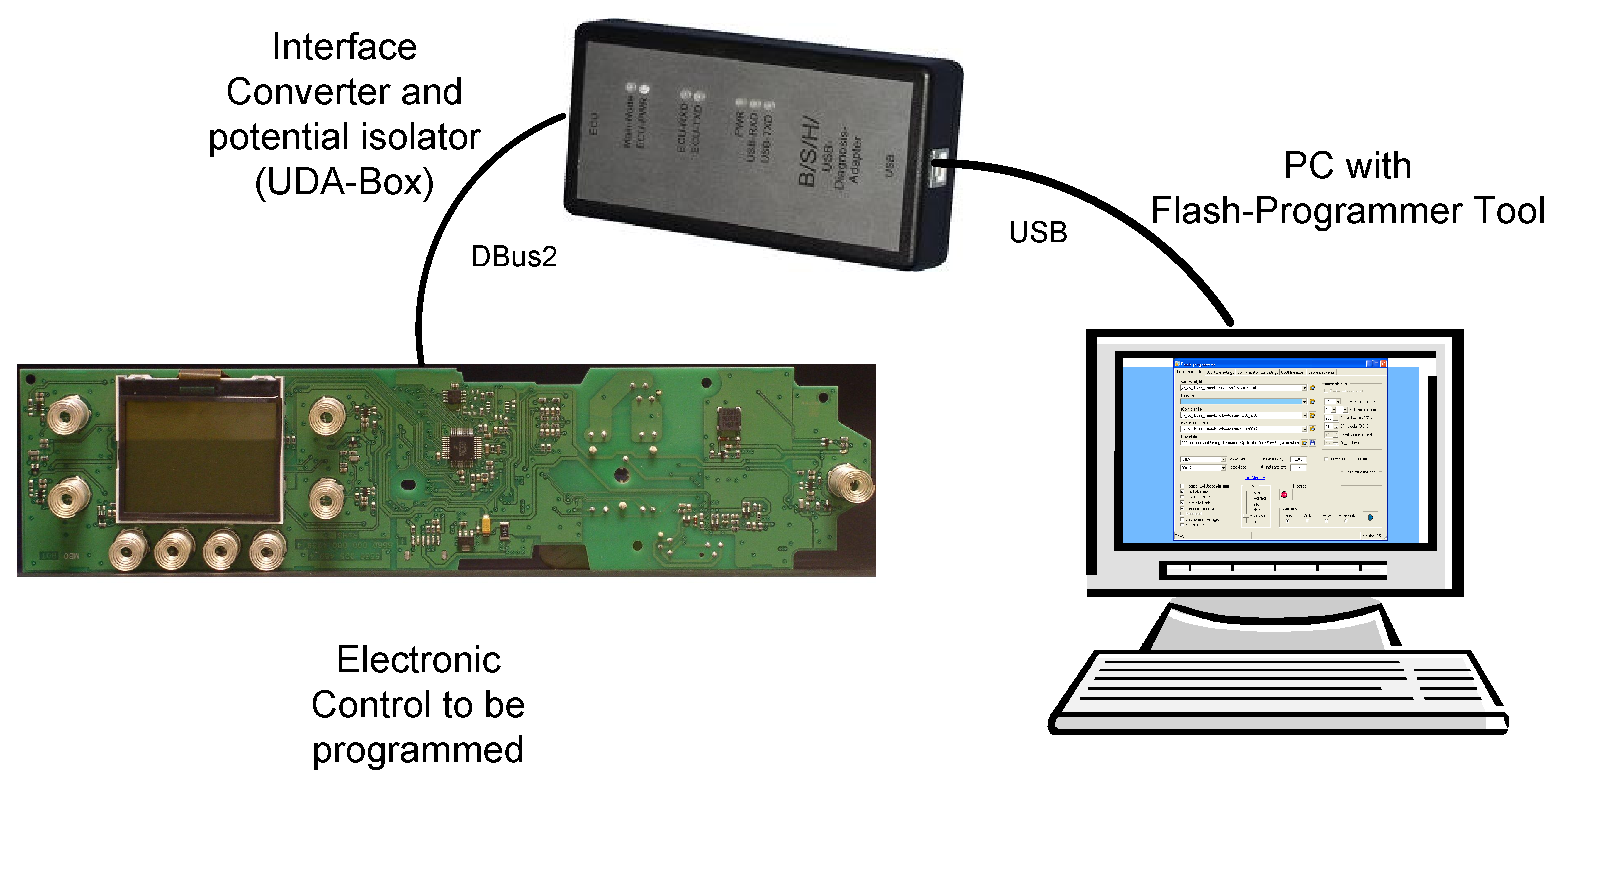
\includegraphics[angle=0,width=16cm]{OverallScheme.eps}
	\caption{Buildup for programming the nonvolatile memory of an electronic control}
	\label{fig:OverallScheme}
\end{figure}


Figure \ref{fig:OverallScheme} shows the required build-up for programming an electronic control. As D-Bus-2 is a multi master bus more than one control may be connected to the bus. The \bl{} protocol just supports a point to point connection. 
To open a point to point connection between the \fp{} and an ECU other communication partners need to ignore the bus messages during update. Therefore a so-called GoOffline message will be sent by the \fp{}.
This message informs the target ECU to be flashed and the others to be quite for time defined in the GoOffline message. For detailed information about this message please refer document \flqq{}BSH General Bus Specification D-Bus-2\frqq{}.
After receiving the GoOffline message the target ECU will perform a reset. After this reset the ROM-\bl{} gets control and sends the boot request (0x54) to the serial interface used for D-Bus-2 also.\footnote{The D-Bus-2 SW is not part of the \bl{}.\\
If no application is present a normal power-on can be used to reset the control. Here as well the \bl{} generates the 0x54 on transmission line.}. For detailed information on startup refer to Chapter \ref{sec:BootloaderStartupSequence}.\\


\subsection{The ROM-\bl}
\label{sec:TheROMBl}
The ROM-\bl{} (\bro{}) is the memory persistent part of the \bl{}. It gets control after reset and sends the boot request (0x54) to a possibly connected \fp{}. If the ROM-\bl{} application does not receive any valid message frame (chapter \ref{sec:BootLoaderMsgFrame}), the \bro{} enters the client application after the boot timeout has been elapsed. Usually some registers of \uc{}-Platforms cannot be rewritten after initialisation (e.g clock or watch dog registers). That's why \bro{} shall use a reset (\emph{fast boot}) to enter the client application. For detailed timeout and reset information refer to Chapter \ref{sec:Timeout} and figure \ref{fig:StateChart}.\\
The second important function of the \bro{} is to load the RAM-Loader \bra{} into RAM. Also the \bro{} supports the change of baud rate (\texttt{SET_BAUDRATE}) and a command to identify the control and \uc{} (\texttt{SELF_IDENT}). Finally the command \texttt{JUMP_LOADER} jumps to the downloaded \bra{}.

\subsection{The RAM-\bl}
\label{sec:TheRAMBl}
The command \texttt{JUMP_LOADER} gives the \bra{} control over the \uc{}. This application supports the commands for erasing programming and reading the flash memory (\texttt{PAGE_ERASE}, \texttt{MASS_ERASE}, \texttt{PROGRAMME_DATA} and \texttt{READ_DATA} ). To leave the \bl{} and get back to the client application the command \texttt{JUMP_APPLICATION} is supported. 
To prevent a deadlock when not all bytes of a message have been received, the \bra{} provides an inter byte timeout. If a message could not be received completely the \bra{} sends the time out acknowledge (see chapter \ref{sec:Acknowledge}).
\footnote{In older versions of \bl -Protocol the \bra{} was responsible to change the baud rate, this is not longer supported as it is handled by the \bro{}.}



\newpage
\subsection{Bootloader Transition State Chart}
The state chart in figure \ref{fig:StateChart} illustrates the interaction between the different applications inside the micro controller including startup and time out.\\
After reset the ROM-Loader gets control. Depending on a special status variable the application will be started or the \bro{} continues.\\
\textbf{Note:} \emph{BootState} must not be initialised during startup, as last saved value should be available after reset.
\begin{figure}[ht]
	\centering
		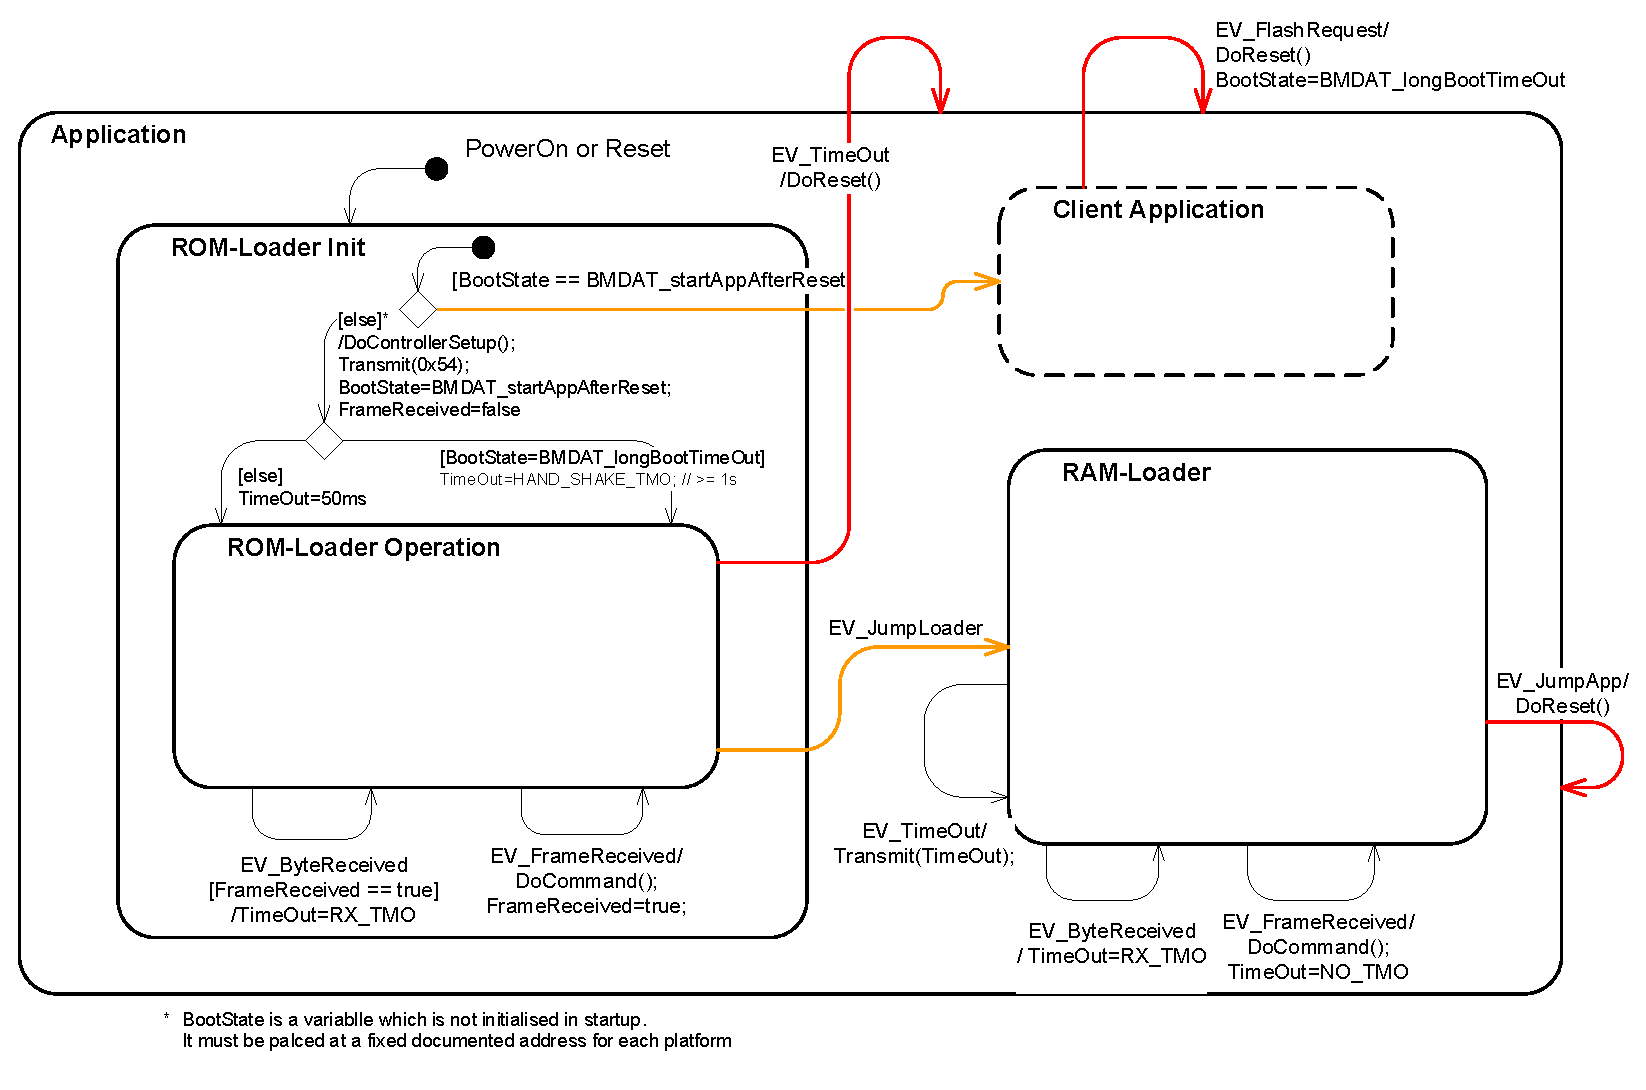
\includegraphics[width=16cm]{BootLoaderHandshake.eps}
	\caption{Transistion State Chart (RAM/ROM-Loader and Application)}
	\label{fig:StateChart}
\end{figure}

\subsubsection{Boot State Variable}
The boot state variable is used to communicate between the application and bootloader. Its content will not be initialized during startup.
The boot state variable is implemented as member \emph{magicPattern} inside the structure \emph{BMDAT_sharedData}. This structure is placed at a common address specified for each platform.
For most platforms this is the first available address inside RAM (0x20000000 for CortexMx and 0x04 for Renesas Rx).
For Cypress/Infineon Psoc4 the structure is placed after the vector table at 0x200000C0.\\
\newpage
\hint{Usually for wired firmware-update the placement of \emph{BMDAT_sharedData} is not that important. When the application does not set the boot state to the value \emph{BMDAT_longBootTimeOut},
there will be the default timeout of romLoader of about 50ms. On extremely slow PCs only this has caused problems in the past.}\\
The Bootloader implementation does not read or set any other attribute than \emph{magicPattern} of \emph{BMDAT_sharedData}!
\lstset{language=C}
\lstset{escapeinside={<@}{@>}}
\begin{lstlisting}[frame=single, basicstyle=\tiny]

enum BMDAT_magicPatterns
{
    BMDAT_startBlAfterReset     = 0x00U,
    BMDAT_longBootTimeOut       = 0x5A5A7979U,
    BMDAT_startAppAfterReset    = 0x55AA7799U,
    BMDAT_magicPattern          = 0x5A714B78U
};

struct BMDAT_sharedData_s
{
    size_t   IsrTableAddress;  // physical address of interrupt vector table
    uint32_t errorFlags;       // error flags
    enum MAL_ModuleEnum errorModule; // module-ID caused an error during booting
    enum MAL_ModuleEnum bootModule;  // identifier of module to boot
    uint16_t baudRate;         // start baud rate for boot loader
    uint16_t startAttempts;    // number of start attempts for boot manager
    uint16_t fatalErrorCounter;// fatal error counter (used in case of functional safety error)
    <@\textcolor{red}{enum BMDAT_magicPatterns magicPattern;}@> // holds a magic pattern to recognize uninitialized data
    enum BMDAT_RamCheckState ramCheckState;// flag for SW/HW reset
};

\end{lstlisting}

\setlength\arrayrulewidth{1pt}
\edsLongtable[]%
   {\rmfamily\textbf{Definition} & \rmfamily\textbf{Value} & & \textbf{Description}}%
   {>{\footnotesize\ttfamily}l >{\footnotesize\ttfamily}r r >{\footnotesize}l}%
   {BMDAT_longBootTimeOut            & 0x5A5A7979   & &  Long handshake timeout requested by application\\
    BMDAT_startAppAfterReset           & 0x55AA7799   & &  \bro{} jumps to application immediately after reset\\
                        & any other      & &  \bro {} will use default hand shake timeout of 50ms\\}
   {Settings for \emph{BMDAT_sharedData.magicPattern}}%
   {tbl:BootState}
\setlength\arrayrulewidth{\arrayrulewidthBak}


\newpage
\subsection{Timeout}
\label{sec:Timeout}
\bro{} and \bra{} support the same message frame, but the requirements for timeout implementation are different.
\subsubsection{ROM-Loader Timeout}
\label{sec:ROMLoaderTimeout}
\paragraph{Hand Shake}
\label{sec:HandShake}
After reset the \bro{} becomes control. Depending on variable \emph{BootState} the client application will be started or different values for timeout are used (figure \ref{fig:StateChart} and Table \ref{tbl:BootState}). The standard hand shake timeout is 50ms. In case of BMDAT_longBootTimeOut this timeout must be at least 1s.\\
The hand shake timeout is active until the first valid frame was received. A valid frame may be also an unknown command. To get fastest communication this first command should be the \texttt{SET_BAUDRATE} command.\\ \textbf{Note:} The \bro{} must not send a \texttt{WRONG_CHECKSUM} or \texttt{TRANSMISSION_ERROR} acknowledge before receiving the first valid message frame, so the first frame will be acknowledged with \texttt{ACKNOWLEDGE_OK} or \texttt{UNKNOWN_COMMAND} if received valid frame has an unknown command.

\paragraph{Message Timeout}
\label{sec:MessageTimeout}
After receiving the first message frame the timer must be loaded with the message timeout which is 250ms. Each received byte reload the timer. If no byte is received during 250ms a reset must be generated to enter the client application.
 
\subsubsection{RAM-Loader Timeout}
\label{sec:RAMLoaderTimeout}
The \bra{} supports an inter byte timeout. This means that between two messages no timeout is generated. After any received byte the timer is loaded with 250ms. If the timer elapsed a \texttt{RECEIVER_TIMEOUT} is sent by the \bra{}. When the last byte of a message was received the timeout is switched off until first byte of next message was received.

\subsection{Bootloader Startup Sequence}
\label{sec:BootloaderStartupSequence}
The sequence in figure \ref{fig:NormalPowerOn} shows the behaviour after a normal power on reset.
After reset the Boot Loader Application becomes the control, as the reset vector points to the \bl-Application. It sends the boot request and sets the fast-boot condition. The fast boot condition will not be cleared during reset (e.g. this can be done by saving it in noninitialised RAM section). When the \fp{} is not present or does not answer (like shown in the figure \ref{fig:NormalPowerOn}), the boot timeout will generate a second reset.\\
After reset the \bl{} starts again, but as fast-boot condition is set the \bl{} jumps immediately to the main application.\\
\begin{figure}[hb]
\resizebox{\linewidth}{!}{%
	\begin{psmatrix}[colsep=0.2,rowsep=0.5]
			[name=flashprog]\umlClass{Flash Prog.}{}
		&	[name=application]\umlClass{Application}{}
		& [name=bl]\umlClass{Boot Loader}{}
		& [name=uc]\umlClass{$\mu{}$Controller}{}		
		\\[0.5cm]
    {} & {} & {} & {}\\
    {} & {} & {} & {}\\
    {} & {} & {} & {}\\
    {} & {} & {} & {}\\
 			[name=flashprogEnd]{}
		&	[name=applicationEnd]{}
		& [name=blEnd]{}
		& [name=ucEnd]{}
		& \\[-0.5cm]
		%
		\ncline[linewidth=0.5pt,linestyle=solid,offset=-1.7,nodesep=0.0]%
    {->}{client}{clientEnd}
    \naput[npos=1]{\emph{t}}
		%
		\ncline[linestyle=dashed]{flashprog}{flashprogEnd}
		\ncline[linestyle=dashed]{application}{applicationEnd}
		\ncline[linestyle=dashed]{bl}{blEnd}
		\ncline[linestyle=dashed]{uc}{ucEnd}
    %
    % Les connexions horisontales ave leur commentaires associ�s
    \small\ttfamily
    \psset{labelsep=1.4mm}
    %
    \ncline{<-}{2,3}{2,4}\naput*{PowerOn()}
    \ncline{<-}{3,1}{3,3}\naput*{SendBootRequest()}
    \ncline{->}{4,3}{4,4}\naput*{TimeOut()}
    \ncline{<-}{5,3}{5,4}\naput*{Reset()}
    \ncline{<-}{5,2}{5,3}\naput*{JumpToApp()}
  \end{psmatrix}
}%end resize
\caption{Normal Power On (\fp{} does not answer)}
\label{fig:NormalPowerOn}
\end{figure}
Figure \ref{fig:BLentry} demonstrate how to initiate the communication between \bl{} and \fp{} using the \dbus{} Go-Offline message. These communication can be started also with a power on reset shown in figure \ref{fig:NormalPowerOn}. As long no timeout happens the \bl{} has the control over the $\mu{}C$. For details of timeout refer chapter \ref{sec:Timeout}.\\
% ---------------------  Boot Loader Entry -------------------------
\begin{figure}
\resizebox{\linewidth}{!}{%
	\begin{psmatrix}[colsep=0.2,rowsep=0.5]
			[name=flashprog]\umlClass{Flash Prog.}{}
		&	[name=application]\umlClass{Application}{}
		& [name=bl]\umlClass{Boot Loader}{}
		& [name=uc]\umlClass{$\mu{}$Controller}{}		
		\\[0.5cm]
    {} & {} & {} & {}\\
    {} & {} & {} & {}\\
    {} & {} & {} & {}\\
    {} & {} & {} & {}\\
    {} & {} & {} & {}\\
    {} & {} & {} & {}\\
    {} & {} & {} & {}\\
 			[name=flashprogEnd]{}
		&	[name=applicationEnd]{}
		& [name=blEnd]{}
		& [name=ucEnd]{}
		& \\[-0.5cm]
		%
		\ncline[linewidth=0.5pt,linestyle=solid,offset=-1.7,nodesep=0.0]%
    {->}{client}{clientEnd}
    \naput[npos=1]{\emph{t}}
		%
		\ncline[linestyle=dashed]{flashprog}{flashprogEnd}
		\ncline[linestyle=dashed]{application}{applicationEnd}
		\ncline[linestyle=dashed]{bl}{blEnd}
		\ncline[linestyle=dashed]{uc}{ucEnd}
    %
    % Les connexions horisontales ave leur commentaires associ�s
    \small\ttfamily
    \psset{labelsep=1.4mm}
    %
    \ncline{->}{2,1}{2,2}\naput*{\dbus::GoOffline()}
    \ncline{->}{3,2}{3,4}\naput*{GenerateReset()}
    \ncline{<-}{4,3}{4,4}\naput*{Reset()}
    \ncline{<-}{5,1}{5,3}\naput*{SendBootRequest()}
    \ncline{->}{6,1}{6,3}\naput*{SendAnyFrame()}
    \ncline{<-}{7,1}{7,3}\naput*{SendAckOK()}
    \ncline{->}{8,1}{8,3}\naput*{SendMoreCommands()}
 
  \end{psmatrix}
}%end resize
\caption{Boot Loader Entry (\fp{} connected)}
\label{fig:BLentry}
\end{figure}
				


\newpage
\section{Boot Loader Protocol}
\label{sec:BootLoaderProtocol}
\subsection{Communication Settings}
The Boot Loader uses the UART based D-Bus-2 interface, but implements a different message stack. To make sure, that the Boot Loader does not accept any D-Bus-2 message from other nodes the Boot Loader protocol uses an even parity. The following table shows the standard communication settings for the UART:\\[0.5cm]
\noindent{}\sffamily
\begin{tabular}{ll}
		\textbf{Baud rate:}   & 9600\\
	  \textbf{Data length:} & 8\\		
		\textbf{Parity:}      & Even\\
		\textbf{Stop bit:}    & 1
\end{tabular}\\[0.5cm]
\normalfont
\textbf{Note:} The Baud rate can be changed using the command \texttt{SET_BAUDRATE}. Also the start baud rate can differ to have e.g. the same baud rate than used for D-Bus-2 protocol.
\pagebreak[0]
\normalfont

\subsection{General Message Frame}
\label{sec:BootLoaderMsgFrame}
The Boot Loader communicate with the Flash Programmer using a simple message frame. This message frame is designed for the UART-based single wire interface of D-Bus-2. Each message is initiated by the Flash Programmer, starting with a sequence of 5 bytes. This frame must be acknowledged by the Boot Loader. The minimal sequence ends with an acknowledge after a 5 byte message frame.\\
The sequence below illustrate a command writing data to the Boot Loader. This diagram and all followings show bytes from Flash Programmer light gray and bytes form the Boot Loader in dark gray color. 

\mkMsgFrame{%
  F|F|F|F|F|L|B|L|F|D|F|F|L|B}{%
  CMD & LEN & ADDH & ADDL & SUM & & ACK & & DAT1 & & DATn & SUM & & ACK}{%
  \cline{2-6}\cline{8-8}\cline{10-10}\cline{12-13} \cline{15-15}
}

\makeTerms{%
CMD 			& Command number.\\
LEN       & Length of data following the command frame (here n bytes to transmit).\\
ADDH/L 	  & High/Low byte of address. Commands which do not need an address with more than 2 data bytes are using this byte for data also (e.g. command \ttfamily{SET_BAUDRATE}).\\
SUM       & Check sum over command frame or data bytes.\\
DAT       & Data byte; may be also transmitted from \bl{} to \fp.\\
}

\subsubsection{Data Length}
\label{sec:DataLength}
For some commands (\texttt{STORE_DATA, PROGRAMME_DATA, READ_DATA}) an explicit data length is required. The maximal supported data length is platform specific and depends on implementation and RAM resources of the \uc{}. The message frame supports a maximum data length of 256 bytes, for these commands a \texttt{LEN=0} means 256 bytes. For all other commands \texttt{LEN=0} means 0 bytes.

\subsubsection{Checksum Calculation}
\label{sec:ChecksumCalculation}

Each command frame or block of data is terminated by the check byte \emph{SUM}. It is an 8-Bit check sum. A possibly overflow (carry) is also added to the sum.\\
	\[SUM +\!= DATi + Carry;
\]
\textbf{Note:} This is the same like performing a sum and then add high- and low-byte. Finally take the low-byte as \emph{SUM}. The check sum never can exceed the 16-bit range.

\subsubsection{Acknowledge}
\label{sec:Acknowledge}
Each command and each data block must be acknowledged by the \bl. There are positive and negative acknowledges. The high nibble of positive acknowledge is always 0xA or 0xB, for negative ones always 0x0. The low nibble of positive acknowledge is also used for an identifier in case of buffered mode\footnote{In older \bl~applications the low nibble of positive acknowledge was used to code the $\mu{}C$ platform, this is not longer required as there is the command \ttfamily{SELF_IDENT}}.

%edsLongtable[x]{headline}{format}{content}{caption}{label}
\setlength\arrayrulewidth{1pt}
\edsLongtable[]%
   {\textbf{\rmfamily{Acknowledge}} & \textbf{\rmfamily{Value}} & & \textbf{Description}}%
   {>{\small\ttfamily}l >{\small\ttfamily}r r >{\small}l}%
   {ACKNOWLEDGE_OK      & 0xA0   & &  Positive acknowledge\\
    FLASH_CMD_OK        & 0xB0   & &  Positive acknowledge for erasing and programming flash\\
    CRC_OK              & 0xC0   & &  Positive acknowledge successful CRC\\
    UNKNOWN_COMMAND     & 0x01   & &  Received command is not supported\\
    WRONG_CHECKSUM      & 0x02   & &  Received checksum was wrong\footnote{May also be answered with \ttfamily{TRANSMISSION_ERROR}.}\\
    SPEED_CH_FAILED     & 0x03   & &  Obsolete, speed check not longer supported\\
    FLASH_CMD_FAILED    & 0x04   & &  Flash command (erasing or flashing) has failed\\
    TRANSMISSION_ERROR  & 0x06   & &  Transmission error  (e.g. parity, overflow $\cdots$)\\
    RECEIVER_TIMEOUT    & 0x07   & &  A timeout happened during receive\\
    CRC_FAILED          & 0x08   & &  CRC error detected\\}%
   {List of defined Acknowledges}%
   {tabAckTbl}
\setlength\arrayrulewidth{\arrayrulewidthBak}

\pagebreak[4]


\subsection{Command Description}
The table \ref{tab:Commands} gives an overview of the supported commands.
The following chapter introduces these commands in detail. As the resources are limited in embedded systems most plausibility checks must be done in the \fp-Application. 
 
%edsLongtable[x]{headline}{format}{content}{caption}{label}
\setlength\arrayrulewidth{1pt}
\edsLongtable[]%
   {\normalfont\small\textbf{Command} & \normalfont\small\textbf{Code} & \small\textbf{Used in} & \small\textbf{Essential} & \small\textbf{Description}}%
   {>{\footnotesize\ttfamily}p{3.0cm} >{\footnotesize\ttfamily}p{1.0cm} >{\footnotesize}m{2.2cm} >{\footnotesize}p{1.6cm} >{\footnotesize}p{5.8cm}}%
   {STORE_DATA          & 0x0A  & BRO            & yes & Stores received data block at the specified address in RAM\\
    JUMP_LOADER         & 0x1A  & BRO            & yes & Does a jump to the specified address, usually to RAM-Loader\\
    SELF_IDENT          & 0x5B  & BRO,\,BP       & no  & Requests the control to identify itself, a ID-String will be transmitted\\
    SET_PAGE            & 0x77  & BRO,\,BRA,\,BP & no  &  Sets the upper 16-bit of a long address\\
    SET_BAUDRATE        & 0x04  & BRO,\,BRA,\,BP & no  &  Change the baud rate\\
    BREAK               & 0x33  & BRA,\,BP       & no  & Breakes a current erase or prigramming command\\
    JUMP_APPLICATION    & 0x02  & BRA,\,BP       & no  &  Jump to the main application using a reset\\
    PAGE_ERASE          & 0x08  & BRA,\,BP       & yes & Erase Flash-ROM page wise\\
    MASS_ERASE          & 0x09  & BRA,\,BP       & no\footnote{At least one of \texttt{PAGE_ERASE}, \texttt{MASS_ERASE} required}
      &  Erase complete flash\\ 
    PROGRAMME_DATA      & 0x18  & BRA,\,BP       & yes &  Programme a block of data in flash memory\\
    READ_DATA           & 0x38  & BRA,\,BP,\,BRO & no  &  Read data from a memory block\\
    CALC_CRC            & 0x39  & BRA,\,BP       & no  &  Performs a CRC and compares to a given one\\
    }
   {Overview: Boot Loader Commands}%
   {tab:Commands}
\setlength\arrayrulewidth{\arrayrulewidthBak}


\noindent{}Table \ref{tab:ObsoleteCommands} shows a list of not longer supported commands. These commands should not be used in future \bl{}~Applications. Due to downward compatibility they must be supported by the \fp.
\setlength\arrayrulewidth{1pt}
\edsLongtable[]%
   {\normalfont\textbf{Command} & \normalfont\textbf{Code} & \textbf{Used in} & \textbf{Description}}%
   {>{\small\ttfamily}p{3.2cm} >{\small\ttfamily}m{1.1cm} >{\small}p{3cm} >{\small}p{6.7cm}}%
    {PROGRAMM_BYTE       & 0x18   & BRA    & Do not use, defined for downward compatibility\\
     READ_DATA32         & 0x39   & BRA    & Read data from the hole memory for reading using 32-bit addresses\\
     PROGRAMM_DATA32     & 0x19   & BRA    & Programme date in Flash-ROM pagewise using 32-bit addresses\\
     STORE_DATA32        & 0x10   & BRO    & Stores received data block at the specified 32-bit address in RAM\\
    }
   {Overview: Obsolete Boot Loader Commands}%
   {tab:ObsoleteCommands}
\setlength\arrayrulewidth{\arrayrulewidthBak}

\subsubsection{Store Data}
\label{sec:CmdStoreData}
This command is provided by the \bro{} to receive the \bra{}~Application, it saves the received data block at the address specified by \emph{ADDH} and \emph{ADDL}. This is an essential command for \bro.\\
\begin{figure}[h]
\begin{center}
\mkMsgFrame{%
  F|F|F|F|F|L|B|L|F|D|F|F|L|B}{%
  0x0A & LEN & ADDH & ADDL & SUM & & ACK & & DAT1 & & DATn & SUM & & ACK}{%
  \cline{2-6}\cline{8-8}\cline{10-10}\cline{12-13} \cline{15-15}
}
\caption{STORE_DATA}
\label{fig:CmdStoreData}
\end{center}
\end{figure}



\subsubsection{Jump Loader}
\label{sec:CmdJumpLoader}
This command is provided by the \bro{} to start the \bra{} after this application it transmitted successfully. The length is unused, although it should be zero \bro{} is not responsible to check this.\\
\begin{figure}[h]
\begin{center}
\mkMsgFrame{%
  F|F|F|F|F|L|B}{%
  0x1A & 0x00 & ADDH & ADDL & SUM & & ACK}{%
  \cline{2-6}% \cline{8-8}   %\cline{10-10}\cline{12-13} \cline{15-15}
}
\caption{JUMP_LOADER}
\label{fig:CmdJumpLoader}
\end{center}
\end{figure}


\subsubsection{Self Ident}
\label{sec:CmdSelfIdent}
This command is a nonessential command provided by \bro{} or \bp. The answer of this read request is an \emph{ID-String} terminated with \texttt{0x55, 0xAA, 0x00}. It returns information about the responsible company, micro controller, protocol revision and optional information about \bl{} variant  and project. Even this command is not essential, it is strongly recommended to implement it. Just for really tiny devices or if an additional flash page can be saved it may be omitted. As the under score is used for separator this symbol may not be used inside any part except the last one (\emph{PN}). The strings should be selected as short as possible. At least 0x20 bytes should be reserved for the ID string including the terminating zero.

\begin{figure}[h]
\begin{center}
\mkMsgFrame{%
  F|F|F|F|F|L|B|B|B|D|B|B|B|B}{%
  0x5B & 0x00 & 0x55 & 0xAA & 0x5B & & ACK & Char1 & Char2 & & 0x55 & 0xAA & 0x00 & SUM}{%
  \cline{2-6}\cline{8-10}\cline{12-15}
}\caption{SELF_IDENT}
\label{fig:CmdSelfIdent}
\end{center}
\end{figure}

\paragraph{Company (CO)}
As the \bl{}-Specification is for external use also, CO specifies the responsible company. For BSH the following strings are recommended: \texttt{GED, PCG, PCP, PDC, PLC, PRF}. For external suppliers it may have any other string e.g. \texttt{AKO, EGO, IST}. Under scores are not allowed inside any string.

\paragraph{Processor Manufacturer (PM)}
This part defines the \uc-Manufacturer. \texttt{`FRE'} for Freescale, \texttt{`REN'} for Renesas, \texttt{`AT'} for Atmel, \texttt{`NEC'} for NEC, \texttt{`ST'} for ST, ...

\paragraph{Processor family and derivative (UC)}
This part identify the the \uc{} family and derivative. E.g. ``S08AC'' for Freescales HCS08AC derivatives. If required also the memory variant must be identified, never the less target is to create as less as possible variants for the boot loaders. 

\paragraph{Protocol version (PV)}
The revision of \bl{}-Protocol.

\paragraph{Boot Loader Version(BV)} This defines a special \bl{} variant.

\paragraph{Project name (PN)}If required also a unique project name can be specified.\\

\vspace{1ex}
\noindent{}So the resulting identification name looks like this:\\
\texttt{CO_PM_UC_PV_BV_PN}\\[1ex]
The last two optional parts may be omitted if not required. Any omitted part must be replaced by under score. The termination in under score is not required if the parts BV and PN are not specified in this string. So \mbox{'\texttt{BSH_FRE_S08AC_2.0}'} is an legal identifier. The last part (PN) may also have under scores inside e.g.:\\
\mbox{'\texttt{BSH_REN_R8C1B_2.0__PH_YL123}'}\\
The \fp{} may use the ID-String to load a specific configuration file.

\subsubsection{Set Page}
\label{sec:CmdSetPage}
The command \texttt{SET_PAGE} is used to set the high word of a long address. This address is used in all following commands as upper part of the address and enable the \bl{} to access also far memory without using 32 bit addresses in the message frame. This is an optional command and just supported for platforms providing far memory. Even when far flash memory is provided, it is not mandatory to support the \texttt{SET_Page} command for \bro{} if only near memory is used.\\
The \bl{} remembers the selected page until a new \texttt{SET_PAGE} frame is received. The default page is zero after reset. \emph{SET_PAGE} expand the address range to 32 bit (4GByte). 
\begin{figure}[h]
\begin{center}
\mkMsgFrame{%
  F|F|F|F|F|L|B}{%
  0x77 & 0x00 & ADDH & ADDL & SUM & & ACK}{%
  \cline{2-6}% \cline{8-8}   %\cline{10-10}\cline{12-13} \cline{15-15}
}
\caption{\texttt{SET_PAGE}}
\label{fig:CmdSetPage}
\end{center}
\end{figure}



\subsubsection{Set Baud Rate}
\label{sec:CmdSetBaudRate}
The command \texttt{SET_BAUDRATE} is an optional command and enables the \fp{} to change the default baud rate. Usually the default baud rate after reset is 9600 baud, but also any other rate is allowed.\\
The two address bytes are used for the baud rate \emph{BDH}, \emph{BDL}. Usually these two bytes are directly copied to the baud rate register of the \uc{}. Many platforms just need a single byte to copy to the baud rate register. In this case just \emph{BDL} is used and \emph{BDH} can be ignored.\\
In most cases it should not be required to calculate the correct register values, therefore the values $0$ is reserved. This value switches to the standard high baud rate (usually 125k baud).\\
As standard baud rates like 115k baud cannot easily reached with simple oscillator frequencies, 125k baud can be used instead. E.~g. a divider of 64 with a bus frequency of 8MHz results in 125k baud. \textbf{The ACK is sent before changing the baud rate!}
 
\begin{figure}[h]
\begin{center}
\mkMsgFrame{%
  F|F|F|F|F|L|B}{%
  0x04 & 0x00 & BDH & BDL & SUM & & ACK}{%
  \cline{2-6}% \cline{8-8}   %\cline{10-10}\cline{12-13} \cline{15-15}
}
\caption{\texttt{SET_BAUDRATE}}
\label{fig:CmdSetBaudRate}
\end{center}
\end{figure}
\newpage
\subsubsection{Break}
\label{sec:CmdBreak}
To interrupt an erasing or programming process this command can be used. Especially for production this may be used to implement flexible timeouts. The \bl{} itself does not provide a command timeout. As not all flash types do support a break of processing this command is not supported for all platforms. Also for derivatives with small resources this command may not be implemented.
 
\begin{figure}[h]
\begin{center}
\mkMsgFrame{%
  F|F|F|F|F|L|B}{%
  0x33 & 0x00 & 0x55 & 0xAA & 0x33 & & ACK}{%
  \cline{2-6}% \cline{8-8}   %\cline{10-10}\cline{12-13} \cline{15-15}
}
\caption{\texttt{BREAK}}
\label{fig:CmdBreak}
\end{center}
\end{figure}



\subsubsection{Jump Application}
\label{sec:JmpApplication}
This command initiates a jump to the application. Usually this is done after flashing is finished, to return to the application. This must be solved using a reset (see also \ref{sec:BootloaderStartupSequence}). As this can also be done using a power on reset, \texttt{JUMP_APPLICATION} is a nonessential command.

\begin{figure}[h]
\begin{center}
\mkMsgFrame{%
  F|F|F|F|F|L|B}{%
  0x02 & 0x00 & 0x55 & 0xAA & 0x02 & & ACK}{%
  \cline{2-6}% \cline{8-8}   %\cline{10-10}\cline{12-13} \cline{15-15}
}
\caption{\texttt{JUMP_APPLICATION}}
\label{fig:CmdJumpApplication}
\end{center}
\end{figure}


\subsubsection{Page Erase}
\label{sec:PageErase}
The command \texttt{PAGE_ERASE} initiates an erase of a single flash page. To interrupt an ongoing flash (after \emph{ACK}, before receiving \emph{FOK}) command the \bl{} provides the optional \texttt{BREAK} command (section \ref{sec:CmdBreak}).\\
The address specified by \emph{ADDH} and \emph{ADDL} is the start address of the page. Where applicable the upper part of address is set by the \texttt{SET_PAGE} command (section \ref{sec:CmdSetPage}).\\
After the page erase process was finished successfully the \bl{} sends the special acknowledge \emph{FOK}. If command buffering is not provided this may also be a normal \emph{ACK}. If erasing failed instead of \emph{FOK} the negative acknowledge \emph{FLASH_CMD_FAILED} is sent. In this case the command sequence must be sent again.
\emph{PAGE_ERASE} is a nonessential command if \emph{MASS_ERASE} is provided. At least one of them is required.\\
\textbf{Note:} This command may also erase the \bro{}.\\ 
\begin{figure}[h]
\begin{center}
\mkMsgFrame{%
  F|F|F|F|F|L|B|D|B}{%
  0x08 & 0x00 & ADDH & ADDL & SUM & & ACK & & FOK}{%
  \cline{2-6}% \cline{8-8}   %\cline{10-10}\cline{12-13} \cline{15-15}
}
\caption{\texttt{PAGE_ERASE}}
\label{fig:CmdPageErase}
\end{center}
\end{figure}

\subsubsection{Mass Erase}
\label{sec:MassErase}
The command \texttt{MASS_ERASE} initiates the erase of complete flash memory. For acknowledge and break handling verify command \texttt{PAGE_ERASE} (\ref{sec:PageErase}).\\
\emph{MASS_ERASE} is a nonessential command if \emph{PAGE_ERASE} is provided. At least one of them is required.\\
\textbf{Note:} This command also erase the \bro{}.\\ 
\begin{figure}[h]
\begin{center}
\mkMsgFrame{%
  F|F|F|F|F|L|B|D|B}{%
  0x09 & 0x00 & 0x55 & 0xAA & 0x09 & & ACK & & FOK}{%
  \cline{2-6}% \cline{8-8}   %\cline{10-10}\cline{12-13} \cline{15-15}
}
\caption{\texttt{MASS_ERASE}}
\label{fig:CmdMassErase}
\end{center}
\end{figure}

\subsubsection{Programme Data}
\label{sec:ProgrammeData}
To programme a block of data into flash memory the command \texttt{PROGRAMME_DATA} is provided. This essential command flashes the received block of data starting with the address specified by \emph{ADDH} and \emph{ADDL}. Where applicable the upper part of address is set by the \texttt{SET_PAGE} command (section \ref{sec:CmdSetPage}). 
For acknowledge and break handling verify command \texttt{PAGE_ERASE} (\ref{sec:PageErase}). In case of non successful programme and also for an interrupted command the according flash memory page must be erased and all blocks inside this block must be programmed again.\\
\textbf{Note:} Before writing the used memory area must be erased.

\begin{figure}[h]
\begin{center}
\mkMsgFrame{%
  F|F|F|F|F|L|B|L|F|D|F|F|L|B|D|B}{%
  0x18 & LEN & ADDH & ADDL & SUM & & ACK & & DAT1 & & DATn & SUM & & ACK & & FOK}{%
  \cline{2-6}\cline{8-8}\cline{10-10}\cline{12-13} \cline{15-15}
}
\caption{\texttt{PROGRAMME_DATA}}
\label{fig:CmdProgrammeData}
\end{center}
\end{figure}

\pagebreak[4]
\subsubsection{Read Data}
\label{sec:ReadData}
Using this command the target memory can be read out. This can be used to perform a verify. Although this is a nonessential command, it is recommended to implement it. For targets with very small RAM this command can also be provided by the \bro{}.\\

\begin{figure}[h]
\begin{center}
\mkMsgFrame{%
  F|F|F|F|F|L|B|B|D|B|B}{%
  0x38 & LEN & ADDH & ADDL & SUM & & ACK & DAT1 & & DATn & SUM}{%
  \cline{2-6}\cline{8-9}\cline{11-12}
}
\caption{\texttt{READ_DATA}}
\label{fig:CmdReadData}
\end{center}
\end{figure}

\pagebreak[3]
\subsubsection{Calculate CRC}
\label{sec:CalcCRC}
This command performs a CRC over the specified address and verify the calculated CRC with the transmitted one. If the calculated and given CRC are equal a positive acknowledge (\emph{COK}) is transmitted. In case of an error the \emph{CRC_FAILED} is transmitted by the \bl{}.\\
Like the \emph{PROGRAMME_DATA} this command starts with a common 5 byte frame, which is followed by the data frame after the \bl{} answers with a positive acknowledge. This is an optional command and the \fp{} must not sent the second part of command in case of \emph(UNKNOWN_COMMAND) acknowledge.
As it may take some time to calculate a CRC, the timeout of \fp{} should be long enough. Also a huge memory block may be splitted into several smaller ones.\\
 
\begin{figure}[h]
\begin{center}
\mkMsgFrame{%
  F|       F|     F|     F|    F|  L|  B}{%
  0x39 & 0x0C & 0x55 & 0xAA & SUM & & ACK}{%
%  \cline{2-6}\cline{8-9}\cline{11-12}
}
\mkMsgFrame{%
   F|    D|  F|      F|    D|   F|     F|   D|   F|    F|   L|  B|  L| B}{%
  ADDH  & &  ADDL & ENDH  & &  ENDL & CRCH & &  CRCL & SUM & & ACK & & COK}{%
  \cline{2-2} \cline{4-5} \cline{7-8} \cline{10-11} \cline{13-13} \cline{15-15}% \cline{11-12}
}


\caption{\texttt{CALC_CRC}}
\label{fig:CmdCalcCrc}
\end{center}
\end{figure}

\pagebreak[4]

\setlength\arrayrulewidth{1pt}
\edsLongtable[]%
   {\normalfont\small\textbf{Parameter}  & \small\textbf{Description}}%
   {>{\footnotesize\ttfamily}p{3.0cm}  >{\footnotesize}p{8cm}}%
   {ADD                 &  Start address of CRC calculation, 32Bit big endian\\
    END                 &  End address of CRC calculation, 32Bit big endian\\
    CRC                 &  Expected CRC, 32Bit big endian\\
    COK                 &  Acknowledge for CRC ok
    }
   {Overview: Parameter CRC-Command}%
   {tab:ParamCRC}
\setlength\arrayrulewidth{\arrayrulewidthBak}

\paragraph{Calculating the expected CRC}
\label{sec:CalculatingTheExpectedCRC}
This document does not describe a particular CRC, as there are hundreds of different types documented. Often a \uc{} supports a specific CRC is solved in hardware. In this case this build-in CRC should be used. The \fp{} must not know the used CRC. The recommended way how to inform the \fp{} about CRC, start and end address is documented in chapter \ref{sec:UsageOfMotorolaSRecords}.


\section{Usage of Motorola S-Records}
\label{sec:UsageOfMotorolaSRecords}
The usage of the Motorola S-Record is not required to use the \bl{} protocol. This section is a proposal for implementation of flash programmers and boot loaders. These proposals are used and implemented by the GED boot loaders and the GED Flash-Programmer.\\
for further details on Motorola S-Record-Format see \cite{SRec}.\\

\subsection{Using the S0-Record for CRC}
\label{sec:UsingTheS0Record}
The S0 record behind the 2 byte address field contains ASCII coded text. Usually a motorola file contains a single S0-Record used for project or variant name and version information. To reduce the length of the S0 record there may be additional S0-Records\footnote{Some tools may have problems with more than one S0-Record}.\\
Also this record may be used to save redundant information e.g. a CRC. A flash programmer may parse this information out of the programming file.\\

\subsubsection{Saving a CRC inside S0-Record}
\label{sec:SavingTheCRCInsideS0Record}
The GED Flash Programmer uses the S0-Record of the programming file to parse control data for the \emph{CALC_CRC}-command.
Table \ref{tab:CRCtags} lists the tags which are defined for the CRC.\\

\setlength\arrayrulewidth{1pt}
\edsLongtable[]%
   {\normalfont\small\textbf{Tag}  & \small\textbf{Description}}%
   {>{\small\ttfamily}p{2.0cm}  >{\small}p{6cm}}%
   {CRCstartX                 &  Start address for CRC calculation\\
    CRCendX                   &  End address for CRC calculation\\
    CRCX                      &  Expected CRC, 32Bit big endian\\
    CRCtmo                    &  Time-out for CRC calculation in seconds.
                                 This is an optional parameter if not present a default value of flash programmer is taken.
    }
   {Tags for CRC-Command with X=1\dots{}n}%
   {tab:CRCtags}
\setlength\arrayrulewidth{\arrayrulewidthBak}

\noindent{}The following text shows an example for a S0-Record content:\\
\begin{flushleft}
\texttt{%
Some text e.g. Project name\\
CRCstart1=0x3000\\
CRCend1=0x3FFF\\
CRC1=0x2433\\
CRCstart2=0x7000\\
CRCend2=0x7FFF\\
CRC2=0x2455\\
CRCtmo=10\\
}
\end{flushleft}

\noindent{}This produces the following S0-Records:
\begin{flushleft}
\texttt{%
S0130000536F6D65207465787420652E672E2050BB\\
S0130010726F6A656374206E616D650A435243733F\\
S013002074617274313D3078333030300A43524356\\
S0130030656E64313D3078334646460A4352433157\\
S01300403D3078323433330A4352437374617274EB\\
S0130050323D3078373030300A435243656E643273\\
S01300603D3078374646460A435243323D30783273\\
S01000703435350A435243746D6F3D313011\\
}
\end{flushleft}

\noindent{}Inside S0-Record tags are separated by the line feed '\bs{}n' (0x0A). Starting a new S0-Record does not produce a line feed.\\
To make the S0 record flexible for future extensions and also easy to parse, the CRC tags can be found in a block starting with \emph{CRCstart1}.
The first non CRC tag terminates parsing of S0 record.

\subsection{Start address of RAM-loader}
The command \emph{JUMP_APPLICATION} needs the start address of the RAM-Loader. This may be a fixed address.\\
BSH GED uses the S9, S7 or S5 record to specify the start address.

%\section{Naming Convention}
\label{sec:NamingConvention}
\subsection{ID-String}
\label{sec:IDString}
\subsection{File Naming}
\label{sec:FileNaming}


\newpage

\begin{landscape}

\section{Remote Firmware Update}
\label{sec:FirmwareUpdate}

If Firmware Update has to be supported the so called Module header has to be added to the ROM-Loader.\\
The ROM-Loader then can be registered in the partition table and will be treated as loadable application. The loadable ROM-Loader is called LRO.\\

Definition of structure for software module header:

\lstset{language=C}

\begin{lstlisting}[frame=single]

struct BMMOD_ModuleHeader
{
    uint32_t       crc_expected;  ///< the crc value of the present module
    const BMMOD_isrPtr_t *ISRtbl_ptr; ///< pointer to start of vector table
    uint32_t       size;             ///< memory used by application incl. sw-header
    uint32_t       executionAddress; /** \brief execution address for the module
                                         usually the physical start address of the module,
                                         in all other cases module will be copied to its
                                         execution address before starting
                                       */
    struct FWU_sw_version_s sw_version; ///< present sw-version
    /** pointer to array of hardware identifiers (for which SW has been build) */
    const struct hw_id_array_s *hw_id_array;
};

\end{lstlisting}

\newpage

Example implementation:

\begin{lstlisting}[frame=single]

SYMBOL_USED const struct BMMOD_ModuleHeader MDHD_ModuleHeader =
{
     /* here must be the result of CRC over requested code area */
    .crc_expected = 0x00, 
     /* start of vector table */
    .ISRtbl_ptr   = ITBL_coreVectors,
    /* size of the module */
    .size         = (size_t)(((FWU_LRO_END_ADDRESS-FWU_LRO_START_ADDRESS)+1u)),
     /* address where to jump BM /without reset */
    .executionAddress = FWU_LRO_START_ADDRESS,
    .sw_version =
    {
     .version =
        {
            .ID = {0},
            .major = {0},
            .minor = {0},
            .revision = {0},
            .build = GIT_WC_HEAD_REV_NUMBER
        }
    },
    .hw_id_array = NULL
};

\end{lstlisting}

\end{landscape}

\newpage

\begin{thebibliography}{widest-label}
\bibitem[1]{MISRA-C} MISRA-2 2004
\bibitem[2]{ANSI-C} ANSI/ISO 9899:1999 - Programming Language C (C99)
\bibitem[3]{PrgC} Programmieren in C, Kernighan/Ritchie
\bibitem[4]{QAC} \url{http://en.wikipedia.org/wiki/QA-C}
\bibitem[5]{NamingConvention}BSH EDS Naming Convention
\bibitem[6]{Doxygen} \url{http://en.wikipedia.org/wiki/Doxygen}
\bibitem[7]{MISRA} \href{http://en.wikipedia.org/wiki/MISRA_C}{http://en.wikipedia.org/wiki/MISRA\_C} and\\ \href{file://RBGNA001/MDisk/QAC/V7.0/m2cm/doc/M2CM-2.1-QAC-7.0-Coding_Standard_Manual.pdf}{MISRA-C (M2CM-2.1-QAC-7.0-Coding\_Standard\_Manual.pdf)}
\bibitem[8]{SRec} \url{http://en.wikipedia.org/wiki/SREC_(file_format)}
\end{thebibliography}

\end{document}


